\documentclass[UTF8]{ctexart}

\usepackage[]{color}

\usepackage{graphicx}  %插入图片的宏包
\usepackage{float}     %设置图片浮动位置的宏包
\usepackage{subfigure} %插入多图时用子图显示的宏包
\usepackage{listingsutf8}   %代码

\usepackage{geometry}  %设置边距
\usepackage{verbatim}  %显示原始字符
\usepackage{cprotect}  % 在标题中显示原始字符

%**********************边距设置****************************************

% \geometry{a4paper,scale=0.8}
\geometry{a4paper,left=2cm,right=2cm,top=2cm,bottom=2cm}


\begin{document}
\title{Git 入门手册}
\author{Liuding.xin}
% \date{}
\maketitle

\begin{abstract}
    本文是记录在学习\LaTeX 过程中遇到的问题和解决办法,并用\LaTeX 写出来。
    真的好困难。
\end{abstract}


\newpage







\section{\LaTeX 笔记}
\subsection{如何在 \LaTeX 中插入代码} % (fold)
\subsubsection{操作步骤} % (fold)

% subsection  (end)
\begin{enumerate}
    \item usepackage Listings

          $\backslash$usepackage\{listingsutf8\}

    \item 设置代码的格式,暂时不错
    \item 在指定的位置插入一下例子
    \label{Code.Insert_pic}
          \begin{lstlisting}[language={tex}]
\begin{figure}[H] %H为当前位置,!htb为忽略美学标准,htbp为浮动图形
\centering %图片居中
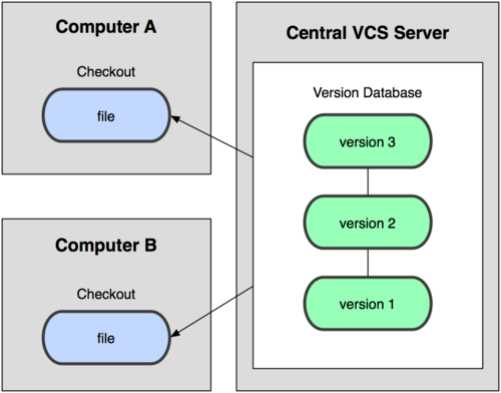
\includegraphics[width=0.7\textwidth]{images/svn-model.png} 
%插入图片,[]中设置图片大小,{}中是图片文件名
\caption{集中化的版本控制系统} %最终文档中希望显示的图片标题
\label{Fig.main2} %用于文内引用的标签
\end{figure}
          \end{lstlisting}


        \end{enumerate}
\subsection{如何在\LaTeX 中插入图片?}
\subsubsection{操作步骤}
插入图片是比较麻烦的时候。不像Word文档那样所见所得。

参考:https://blog.csdn.net/chichoxian/article/details/52588833

\begin{enumerate}
    \item 插入代码,参考代码\ref{Code.Insert_pic}
    \item 最终效果,图\ref{Fig.insert-one-png}
          \begin{figure}[H] %H为当前位置,!htb为忽略美学标准,htbp为浮动图形
              \centering %图片居中
              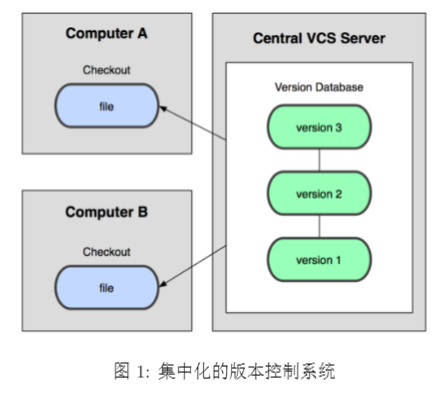
\includegraphics[width=0.5\textwidth]{images/insert-png.png} %插入图片,[]中设置图片大小,{}中是图片文件名
              \caption{插入图片的demo} %最终文档中希望显示的图片标题
              \label{Fig.insert-one-png} %用于文内引用的标签
          \end{figure}

    \item 双排设置
          \begin{lstlisting}
Figure \ref{Fig.main} has two sub figures, fig. \ref{Fig.sub.1} is the travel demand of driving auto, and fig. \ref{Fig.sub.2} is the travel demand of park-and-ride.

\begin{figure}[H]
\centering  %图片全局居中
\subfigure[name1]
{
    \label{Fig.sub.1}
    \includegraphics[width=0.45\textwidth]{DV_demand}
}
\subfigure[name2]
{
    \label{Fig.sub.2}
    \includegraphics[width=0.45\textwidth]{P+R_demand}
}
\caption{Main name}

\label{Fig.main}
\end{figure}
        \end{lstlisting}

    \item 双排效果显示,图 \ref{Fig.Insert_two_pic_demo}
          \begin{figure}[H]
              \centering
              %插入图片,[]中设置图片大小,{}中是图片文件名
              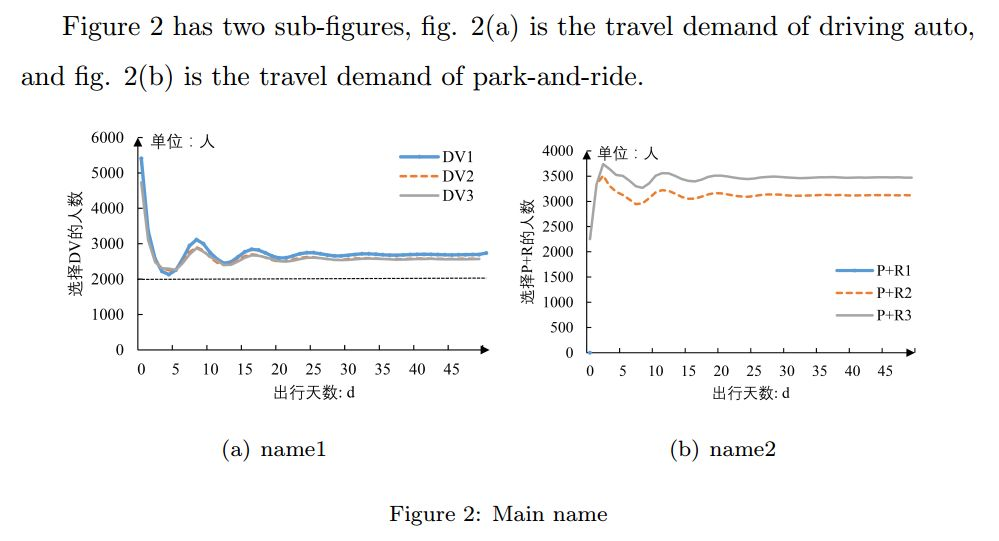
\includegraphics[width=1.0\textwidth]{images/insert-two-pic.jpg}
              \caption{并排插入两个图片的效果}
              \label{Fig.Insert_two_pic_demo}
          \end{figure}

    \item 引用图片

    在文档中使用$\backslash$ref\{标签\},如\verb!\ref{Fig.insert-one-png}!

\end{enumerate}








\subsection{如何设置边距}
\subsubsection{操作步骤}
\begin{enumerate}
    \item 引用geo 设置宏包
          $\backslash$usepackage\{geometry\}
    \item 设置页边距
          \begin{enumerate}
              \item 设置为缩放的形式

                    $\backslash$geometry\{a4paper,scale=0.8\}
              \item 设置为绝对距离

                    $\backslash$geometry\{a4paper,left=2cm,right=2cm,top=2cm,bottom=2cm\}
          \end{enumerate}
    \item 效果不错
\end{enumerate}

\cprotect\subsection{如何输出反斜杠"\verb!\!"?}
要想打印 "\verb!\!" 比较麻烦。参考 https://blog.csdn.net/xovee/article/details/106728213
\begin{enumerate}
    \item 文本中

          \begin{enumerate}
              \item 使用\verb!\!verb!\verb!\!!,注意是"!!" 之间进行截止
              \item 使用\verb!$\backslash$!
              \item 使用代码
                    \begin{lstlisting}{language=tex}
\usepackage{verbatim}
\begin{verbatim} % 使用代码的的形式显示
    \
\end{verbatim}
                    \end{lstlisting}
          \end{enumerate}

    \item 标题中

          1. 引用 cprotect 宏
          \begin{lstlisting}
\usepackage{cprotect}
% 在标题中显示原始字符
            \end{lstlisting}

          2. 在 标题中插入
          \begin{lstlisting}
\cprotect\section{This is a section heading with a verbatim \verb!\frac{1}{2}!}
% 这是在标题中使用\verb
          \end{lstlisting}

\end{enumerate}

\end{document}